\documentclass[../main.tex]{subfiles}

\begin{document}
\chapter{Menyimpan Banyak Data - Array}
\section{Motivasi}
Jika program digunakan hanya untuk memproses data yang dapat dihitung dengan
jari, kenapa kita menggunakan program untuk memprosesnya? Salah satu kemampuan
komputer adalah mengolah data dalam jumlah besar, sehingga lebih efisien dan
lebih tidak mudah \eng{error}. Untuk memproses data yang banyak, pasti butuh
tempat yang dapat menampung data yang akan diproses dan juga data yang sudah
diproses. Di sini tempat \eng{Array} digunakan.

\section{Array 1-dimensi}
Cara mendeklarasi \eng{array} sama dengan cara mendeklarasikan variabel pada
umumnya, hanya saja ada sedikit tambahan \eng{syntax} untuk menentukan variabel
itu sebuah \eng{array}.

\begin{minted}{cpp}
char huruf[26];
int nilai[5] = {19, 8, 9, 12, 97};
\end{minted}

\begin{figure}[h]
\centering
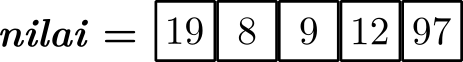
\includegraphics[scale=0.5]{img/array_1_dec_init}
\caption{Visualisasi deklarasi dan inisialisasi \eng{array}}
\label{arr:decinit}
\end{figure}

Nilai dalam \eng{array} diakses dengan memanggil nama variabel ditambah indeks
penyimpanan \eng{array}. Indeks \eng{array} dalam C++ dimulai dari \(0\). Jika
terdapat \eng{array} dengan \(5\) kolom, indeks terakhir adalah \(4\).

\begin{minted}{cpp}
int nilai[5];
nilai[0] = 42;
nilai[4] = 0;
nilai[1] = nilai[4];
\end{minted}

Program di bawah mencontohkan cara penggunaan \eng{array} untuk menyimpan data
yang dimasukkan dan menampilkan data tersebut.

\cppfile{code/contoh_array.cpp}

\section{Array n-dimensi}
\eng{Array} juga bisa digunakan untuk menyimpan data yang terdiri dari kolom dan
baris (\eng{array} \(2\) dimensi), ataupun \(n\)-dimensi. Contoh pembuatan
\eng{array} 2 dimensi;

\begin{minted}{cpp}
char papan[3][3];
int data[5][4][3];
\end{minted}

\begin{figure}[h]
\centering
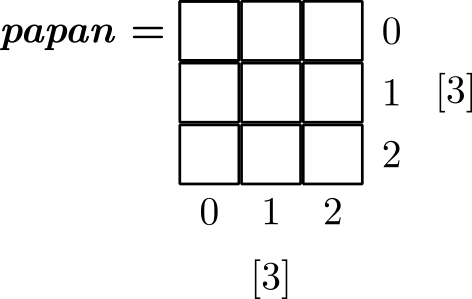
\includegraphics[scale=0.5]{img/array_2_vis}
\caption{Visualisasi \eng{array} 2 dimensi}
\label{arr:2vis}
\end{figure}

\paragraph{Latihan}
\begin{enumerate}
	\item Buat sebuah program yang menampilkan deret Fibonacci. Gunakan \eng{array} untuk menyimpan datanya.
	\item Buat sebuah program yang mengurutkan isi dari array.
\end{enumerate}
\end{document}
